\chapter{Lenguaje Natural}
\label{cap:Lenguaje_Natural}

Tras explorar en el capítulo anterior la arquitectura del transformador y su mecanismo de autoatención, nos adentramos ahora en su mayor caso de éxito: la revolución del Procesamiento del Lenguaje Natural (NLP). El diseño del transformador superó las limitaciones de los modelos clásicos, permitiendo procesar grandes secuencias de texto en paralelo y capturar el contexto de las palabras con una eficacia sin precedentes.

Sin embargo, el verdadero punto de inflexión llegó de la mano de OpenIA en su influyente artículo \textit{Scaling Laws for Neural Lenguage Models} \cite{kaplan2020scaling}, donde demostraron empíricamente que el rendimiento de los modelos de lenguaje mejoraban según aumentaban el tamaño de la red, la capacidad de cómputo y, sobre todo, el volumen de los datos. Al llevar este escalado a niveles masivos, nacieron los \textit{Large Lenguage Models} (LLMs) o, en español, los modelos extensos de lenguaje. Gracias a este crecimiento, se observó que redes entrenadas únicamente para predecir la siguiente palabra desarrollaron una profunda ``comprensión'' de la sintaxis y la semántica y dejaron de ser sistemas especializados en una tarea para convertirse en herramientas de propósito general, capaces de traducir, resumir o razonar con apenas unas instrucciones (los famosos \textit{prompts)}.

Con todo ello, resulta fundamental entender qué ocurre exactamente en el interior de 
estos modelos extensos del lenguaje y cómo se utilizan según el problema que 
queramos resolver. En este capítulo explicaremos en detalle cómo se procesa el 
lenguaje natural dentro de los LLMs; abordaremos cómo se transforma el texto bruto 
en vectores mediante la tokenización y los \textit{embeddings}, y analizaremos varias  
estructura de los transformadores, entre ellas, las estructuras autorregresivas que 
impulsan la actual inteligencia artificial generativa.


%==========================================
%TOKENIZACION
%==========================================
\section{Tokenización}

El primer paso en el procesamiento del lenguaje es transformar el texto en bruto en un formato estructurado que el modelo pueda interpretar. Para ello, es necesario definir un \textbf{vocabulario}: un conjunto finito de unidades básicas de texto que el modelo es capaz de reconocer y procesar.

Una primera aproximación para definir este vocabulario consistiría en utilizar 
únicamente caracteres individuales: letras, números y signos de puntuación. 
Sin embargo, este enfoque presenta desventajas significativas pues aislar los 
caracteres destruye la semántica del lenguaje y dificulta la comprensión real del 
texto, por no mencionar que genera secuencias de entrada excesivamente largas 
(por ejemplo, este pequeño párrafo contiene ya $439$ caracteres). Otra aproximación 
sería considerar un diccionario literal compuesto exclusivamente por palabras enteras. 
No obstante, este método es poco flexible, pues si el modelo recibiese una palabra 
que no está en su vocabulario, como un nombre propio o un error ortográfico, el 
modelo sería incapaz de procesarlo.

Para resolver esta dicotomía, se emplea el proceso de \textbf{tokenización}. 
Este método busca un equilibrio dividiendo el texto de entrada en unidades más pequeñas
llamadas \tokens{}, que formarán el vocabulario y serán lo que realmente reciba y 
procese el transformador como entrada. Estos \tokens{} pueden ser palabras enteras que 
suelen aparecer con mucha frecuencia, caracteres individuales o fragmentos de 
palabras (raíces o terminaciones).
Para  entender las ventajas de usar \tokens{} consideremos las palabras 
\textit{cocinar}, \textit{cocinado}, \textit{cocinero} y \textit{cocina}. 
Todas ellas comparten la misma raíz \textit{cocin-}. Mediante la tokenización, 
resulta mucho más práctico considerar \textit{cocin-} como un \token{} independiente 
perteneciente al vocabulario y, de este modo, interpretar el resto de palabras como 
la concatenación de dicha raíz con sus correspondientes sufijos que, a su vez, 
serán \tokens{} independientes o concatenaciones de otros \tokens{}.

Este proceso de tokenización otorga al modelo la flexibilidad deseada pues en 
lugar de fallar ante palabras nuevas o desconocidas, el modelo los divide en \tokens{} 
que sí pertenecen a su vocabulario y que, en consecuencia, sí es capaz de procesar. 

Surge entonces la cuestión fundamental de cómo se definen y obtienen dichos \tokens{}. 
Existen varios métodos, pero el más famoso y el más utilizado es mediante el algoritmo 
de \textbf{Codificación de Pares de Bytes} (\textit{Byte Pair Encoding}): 

\begin{algorithm*}
    \caption{Algoritmo de codificación de pares de bytes (BPE)}
    \label{alg:bpe}
    \begin{algorithmic}[1]
    \Require Cadena de texto $\mathcal{S}$ y tamaño de vocabulario requerido $k$.
    \Ensure Vocabulario $\mathcal{V}$ de \tokens{}.
    \State Inicializar $\mathcal{V}$ como el conjunto de todos los caracteres individuales únicos en $\mathcal{S}$.
    \State Reemplazar todos los espacios en $\mathcal{S}$ con un \token{} especial de espacio.
    \While{$|\mathcal{V}| < k$}
        \State Encontrar el par de \tokens{} adyacentes $t_1, t_2$ más frecuente en $\mathcal{S}$.
        \State Definir un nuevo \token{} $t_{\text{nuevo}} = Concatenar(t_1,t_2)$.
        \State Añadir $t_{\text{nuevo}}$ a $\mathcal{V}$.
        \State Reemplazar todas las ocurrencias del par $t_1, t_2$ en $\mathcal{S}$ con $t_{\text{nuevo}}$.
    \EndWhile
    \State \Return $\mathcal{V}$
    \end{algorithmic}
\end{algorithm*}
La idea del algoritmo es la siguiente: partimos de un texto $\mathcal{S}$ y 
un valor $k$ que representará el tamaño de nuestro vocabulario $\mathcal{V}$, 
donde los \tokens{} iniciales que componen $\mathcal{V}$ son todos los caracteres 
distintos que aparecen en $\mathcal{S}$. En cada iteración, el algoritmo busca el 
par de \tokens{} consecutivos que aparece con mayor frecuencia y acto seguido los 
fusiona para crear un \token{} nuevo que se añade al vocabulario y actualiza el texto 
original reemplazando el par separado con el nuevo \token{}. Este proceso se repite 
sucesivamente durante $k$ iteraciones (ver figura \ref{fig:bpe}).

Observamos que este algoritmo depende mucho del texto de entrada $\mathcal{S}$, 
por lo que es imprescindible partir de un corpus de entrenamiento masivo que 
represente el dominio sobre el que operará el modelo. Por ejemplo, si el objetivo es 
desarrollar un sistema especializado en derecho, resulta útil que el corpus esté 
compuesto por la mayor cantidad de textos jurídicos. De este modo, el algoritmo 
aprenderá a agrupar los caracteres en raíces y terminaciones más frecuentes de dicha 
jerga.

En la práctica el vocabulario $\mathcal{V}$ es un diccionario clave-valor donde 
cada \token{} tiene asociado un identificador numérico único. Además, es muy 
importante tener en cuenta que  el carácter que representa el espacio en blanco no 
se omite, sino que se incluye en $\mathcal{V}$ como un \token inicial. De esta manera 
el modelo puede aprender a distinguir si una secuencia de caracteres forma una palabra 
independiente o si es un fragmento. Generalmente, el espacio en blanco suele estar 
concatenado al inicio de ciertos \tokens{} (ver figura \ref{fig:tokenizadores}).


\begin{figure}[t]
    \centering
    \BPE
    \caption{Ejemplo de $5$ iteraciones de BPE sobre una frase. Inicialmente el vocabulario $\mathcal{V}$ está formado por los caracteres que componen la frase. En la primera iteración se busca el par de \tokens{} consecutivos más frecuente que, en este caso, son ``o'' e ``y''. Estos dos nuevos \tokens{} forman un \token{} nuevo ``oy'' que se añade a $\mathcal{V}$. Después, en la segunda iteración, se tiene que los \tokens{} ``e'' y ``s'' son el par consecutivo más frecuente, y, en consecuencia, se añade un nuevo \token{} ``es'' al vocabulario. En la tercera iteración, el par de \tokens{} consecutivos más frecuente son ``h'' y ``oy'', luego, repitiendo el mismo proceso, se añade un nuevo \token{} ``hoy'' a $\mathcal{V}$. Finalmente, el vocabulario resultante será la unión de los caracteres que conforman la frase inicial con el conjunto $\{ \text{oy, es, hoy, ya} \}$. Destacar que no hay un criterio estandarizado para resolver los empates en las frecuencias y en este ejemplo, en caso de empate, se ha elegido aleatoriamente el par más frecuente.}
    \label{fig:bpe}
\end{figure}

%==========================================
%IMAGENES EJEMPLO TOKENIZER
%==========================================

\begin{figure}[htbp] 
     \centering       
    % --- PRIMERA IMAGEN ---
    \subfloat[Vocabulario GPT2 de $50.000$ \tokens{}\label{subfig:imagen_a}]{
        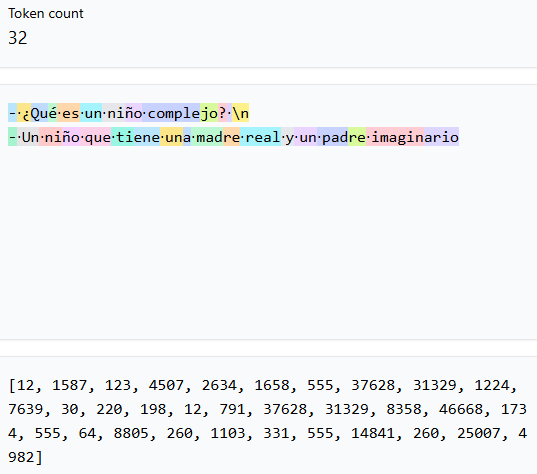
\includegraphics[width=0.60\textwidth]{Imagenes/gpt2_ej.png}
    }% 
    \hfill
    % --- SEGUNDA IMAGEN ---
    \subfloat[Vocabulario \textit{cl100k\_base} de $100.000$ \tokens{} \label{subfig:imagen_b}]{
        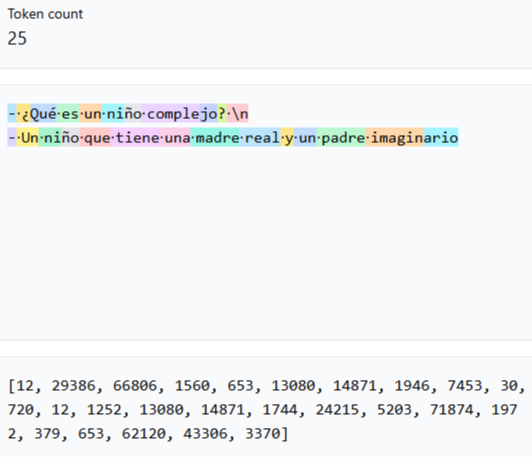
\includegraphics[width=0.60\textwidth]{Imagenes/clk_100_ej.png}
    }

    \vspace{1em} 
    \caption{Comparación visual de la fragmentación de tokens entre los vocabularios de GPT-2 y GPT-4 (cl100k\_base). El número de \tokens{} para la misma frase es distinto. También se observa que en a) la palabra \textit{madre} se compone de dos \tokens{}, mientras que en b) es un \token{} entero. En ambos el punto representa el espacio en blanco y los \tokens{} que suelen representar el inicio de una palabra van precedidos por el punto. Los vectores de números representan los identificadores de cada \token{} en orden y se observa que \tokens{} iguales como ``$\cdot$¿'' tienen distinto identificador: 1587 en a) y 29386 en b). Imágenes obtenidas a través de \url{https://tiktokenizer.chatgptcn.com/}, herramienta interactiva donde se puede observar cómo tokenizan distintos vocabularios.}
    \label{fig:tokenizadores} 
\end{figure}


%==========================================
%EMBEDDINGS
%==========================================

\section{\textit{Embeddings}}

Una vez definido el vocabulario y comprendido el proceso de tokenización, el siguiente paso natural es convertir dichos \tokens{} en un formato que la red neuronal pueda procesar. Como se ha comentado en la sección anterior, los \tokens{} pertenecientes a un vocabulario $\mathcal{V}$ son, inicialmente, simples identificadores numéricos. Sin embargo, tal y como se introdujo al inicio de la sección \ref{procesamiento}, el transformador opera con vectores
$\x_n^T = ( \x_{n1}, \x_{n2}, \dots,\x_{nD_i})$
a los que también llamábamos \tokens{}. Con todo ello, es necesario realizar una transformación que asigne a  un identificador un vector.

Supongamos entonces un vocabulario $\mathcal{V}$ de cardinal $k$. 
Definiremos una matriz $\textbf{E}$, denominada matriz de \textit{embedding}, 
de dimensión $D_i \times k$. 
Además, cada \token{} de $\mathcal{V}$ será representado mediante un 
vector $t_n^T$ =  $(0, \dots,1, \dots,0) \in \mathbb{R}^k$ formado por $0$'s salvo 
la posición $n$-ésima donde vale $1$ y  representará el \token{} $n$-ésimo. 
Finalmente, realizamos la siguiente transformación lineal:
\begin{equation}
    \x_n = \textbf{E} t_n \in \mathbb{R}^{D_i}
    \label{token}
\end{equation}
donde $\x_n$ es el \token{}  $n$-ésimo que procesará el transformador y al que 
hacíamos referencia en la sección \ref{procesamiento}.

Cabe señalar que representar los \tokens{} de $\mathcal{V}$ solo con vectores de la 
base canónica no es práctico, pues, por lo general, $\mathcal{V}$  suele estar 
compuesto por cientos de miles de \tokens{} y los vectores $t_n$ serían 
dimensionalmente muy grandes. Además, lo habitual es considerar $D_i \leq k$, 
reduciendo así la dimensión de $\x_n$. Por otro lado, los vectores canónicos no 
capturan ningún tipo significado o semántica y mucho menos relaciones entre \tokens{}, 
ya que se trata de vectores ortogonales entre sí. En consecuencia, 
la matriz $\mathbf{E}$ se define como una matriz de parámetros entrenables y cuyos 
pesos se van ajustando durante el entrenamiento junto al transformador. 
De aquí en adelante cuando hagamos referencia a los \tokens{} pensaremos siempre 
en  \eqref{token}.
\begin{figure}[t]
    \centering
    \embeddingflujo
    \caption{Procesamiento del texto hasta llegar al transformador.}
    \label{fig:embeddingflujo}
\end{figure}
%==========================================
%transformadorES
%==========================================
\section{Transformadores}
Hasta ahora hemos visto cómo la información se procesa y convierte en vectores de $\mathbb{R}^{D_i}$  para que el transformador sea capaz de asimilarla e interpretarla y, sobre todo, comprendemos la arquitectura general del transformador. En consecuencia, en esta sección abordaremos cómo se adapta la arquitectura y tratamos esa información preprocesada dependiendo de la tarea específica que queramos resolver. Para ello, estudiaremos tres variantes principales: codificador (\textit{encoder}), decodificador (\textit{decoder}) y codificador-decodificador (\textit{encoder-decoder}).

El codificador (\textit{encoder}) procesa la secuencia de entrada en su totalidad para extraer una representación interna de alta dimensionalidad y actúa como un extractor de características diseñado para clasificar o analizar texto, tales como el análisis de sentimientos o el reconocimiento de entidades.

Por otro lado, el decodificador (\textit{decoder}) es un modelo puramente generativo cuya finalidad es la construcción de nuevas secuencias de forma autorregresiva. Para garantizar un aprendizaje coherente, esta variante emplea un mecanismo de atención enmascarada que impide al modelo acceder a información de posiciones futuras. De este modo, la predicción de cada nuevo elemento se realiza basándose exclusivamente en los tokens generados con anterioridad. 

Finalmente, la arquitectura  codificador-decodificador (\textit{encoder-decoder}) 
es una estructura híbdrida de las anteriores concebida específicamente para 
problemas de secuencia a secuencia. En este esquema, el proceso se divide en dos 
fases complementarias: mientras el codificador genera una representación matemática 
global de la entrada, el decodificador produce la salida apoyándose no solo en su 
propia entrada, sino también en la información estructurada que le transfiere el 
codificador a través del mecanismo de atención cruzada (\textit{cross-attention}).
Esta interconexión es la que permite resolver con éxito tareas de alta complejidad 
donde el significado debe preservarse íntegramente entre distintos dominios, siendo 
la traducción automática de idiomas el ejemplo más representativo de su aplicación.

%==========================================
%DECODERS
%==========================================

\subsection{Decodificador}

Los decodificadores son un tipo de arquitectura cuyo propósito principal es 
funcionar como modelos generativos para crear o generar secuencias de \tokens{}. 
Pertenecen a la familia de los denominados \textit{modelos autorregresivos}: modelos 
probabilísticos diseñados para procesar datos secuenciales, donde la probabilidad de 
que aparezca un elemento en la secuencia depende de los elementos que lo precedieron.

\subsubsection{Probabilidad Condicionada}
El objetivo principal de un modelo autoregresivo es, dada una secuencia de \tokens{}
$\x_1, \dots, \x_n$, calcular la probabilidad conjunta $p(\x_1, \dots, \x_n)$. Esta probabilidad, desarrollando mediante la probabilidad condicionada, resulta en:
\begin{equation}
    p(\x_1, \dots, \x_n) = \prod_{t=1}^{n}p( \x_t | \x_1, \dots, \x_{t-1})
\end{equation}
Por lo tanto, calcular la probabilidad conjunta de toda la secuencia se traduce en calcular las correspondientes probabilidades condicionadas. Y esta es exactamente la tarea fundamental que realizan los modelos autorregresivos y, en nuestro caso, el decodificador.

Nuestro objetivo es, por tanto, adaptar la salida del transformador para que 
funcione como un modelo autorregresivo. En otras palabras, buscamos traducir 
su salida a una distribución de probabilidades sobre un 
vocabulario $\mathcal{V}$. 
Para ello, recordemos que a nivel interno el transformador mapea una secuencia 
de \tokens{} $\x_1, \dots, \x_n$ en una secuencia de  vectores 
$\widetilde{\x}_1, \dots, \widetilde{\x}_n$ de dimensión $D_i$. Sin embargo, 
para que el decodificador pueda predecir el siguiente elemento, necesitamos que 
su salida sea una distribución sobre un vocabulario $\mathcal{V}$ de tamaño $k$, 
la cual determine la probabilidad que tiene cada \token{} de continuar la 
secuencia, es decir, necesitamos modificar la salida del transformador  en una
distribución de probabilidad. 
Para lograr esto, realizaremos una transformación lineal utilizando una matriz de 
pesos $\mathbf{\Omega}_o$ de 
dimensión $D_i \times k$, seguida de la función de activación Softmax:
\begin{equation}
    \mathbf{Y} = \text{Softmax}[\widetilde{\mathbf{X}}\mathbf{\Omega}_o]
\end{equation}
donde $\mathbf{Y}$ tiene dimensión $n \times k$ y $\widetilde{\mathbf{X}}$ es 
la matriz cuyas filas son la salida $\widetilde{\x}_1^T, \dots, \widetilde{\x}_n^T$
del transformador. 
Al aplicar la función Softmax, garantizamos que cada una de las filas $\y_j^T$ 
contenga elementos comprendidos entre 0 y 1, y que su suma total sea 
exactamente uno. Dicho de otra manera, cada fila se transforma en una distribución 
de probabilidad válida. 
Por lo tanto, la fila $j$-ésima $\y_j^T$ de $\mathbf{Y}$ representa la 
distribución de probabilidades sobre el vocabulario $\mathcal{V}$ para predecir 
el siguiente \token{}, condicionada por la subsecuencia de 
\tokens{} procesada hasta ese momento $\x_1, \dots, \x_j$ (con $j \leq n$):
\begin{equation*}
\resizebox{\textwidth}{!}{%
$\mathbf{Y} =
\begin{pmatrix}
p(\x_2 = v_1 \mid \x_1) & p(\x_2 = v_2 \mid \x_1) & \dots & p(\x_2 = v_k \mid \x_1) \\
p(\x_3 = v_1 \mid \x_1, \x_2) & p(\x_3 = v_2 \mid \x_1, \x_2) & \dots & p(\x_3 = v_k \mid \x_1, \x_2) \\
\vdots & \vdots & \ddots & \vdots \\
p(\x_{n+1} = v_1 \mid \x_1, \dots, \x_n) & p(\x_{n+1} = v_2 \mid \x_1, \dots, \x_n) & \dots & p(\x_{n+1} = v_k \mid \x_1, \dots, \x_n)
\end{pmatrix}$%
}
\end{equation*}
donde $\x_{n+1}$ representa la predicción del siguiente \token a toda la secuencia 
$(\x_1, \dots, \x_n)$.

Sin embargo, si observamos detenidamente la matriz $\mathbf{Y}$ y recordamos 
cómo funciona el proceso de autoatención, nos damos cuenta de un problema 
estructural: no podemos asegurar que las probabilidades condicionadas dependan 
exclusivamente de los \tokens{} procesados hasta la posición $j$. 
Dado que la atención procesa toda la secuencia en paralelo y atiende a todos los 
elementos simultáneamente, al calcular la salida $\widetilde{\x}_j$, el modelo 
tendría acceso a la información de los \tokens{} futuros ($\x_{j+1}, \dots, \x_n$).
Si entrenásemos al modelo así, simplemente aprendería a hacer trampas: 
``miraría'' el texto adelantado y copiaría la respuesta en lugar de aprender a 
predecirla.
Para evitar esto y garantizar que la arquitectura funcione correctamente como 
un modelo autorregresivo, es necesario introducir una modificación en el proceso: 
la autoatención enmascarada (\textit{masked self-attention}).


\subsubsection{Autoatención Enmascarada}
Para garantizar matemáticamente que cada fila $j$ de la matriz $\mathbf{Y}$ 
represente una verdadera distribución condicionada de manera exclusiva a los 
\tokens{} previos, debemos impedir que el \token{} $\x_j$ ``mire hacia el futuro''.
Queremos asegurar que, al procesar la secuencia, un \token{} en la posición $j$ 
solo calcule su atención basándose única y exclusivamente en sí mismo y en 
los \tokens{} que lo preceden, ignorando por completo la posición $j+1$ y 
posteriores. Dado que los \tokens{} fluyen de manera independiente por el 
transformador y el único punto donde intercambian información es durante el 
cálculo de los coeficientes de atención ($\mathbf{Q} \mathbf{K}^T$), 
es precisamente en esta operación donde debemos intervenir.

Se introduce entonces una matriz de enmascaramiento, denotada como $\mathbf{M}$, 
de dimensión $N \times N$, donde $ N$ representaba el número de \tokens{} que 
recibía el transformador como entrada. Esta matriz presenta la siguiente 
estructura:
\begin{equation*}
    \mathbf{M} = \begin{pmatrix} 
0 & -\infty & -\infty & \cdots & -\infty \\ 
0 & 0 & -\infty & \cdots & -\infty \\ 
0 & 0 & 0 & \cdots & -\infty \\
\vdots & \vdots & \vdots & \ddots & \vdots \\ 
0 & 0 & 0 & \cdots & 0 
\end{pmatrix}
\end{equation*}
La matriz $\mathbf{M}$ se suma a la atención calculada justo antes de aplicar la función Softmax:
$$\text{Softmax}\left[ \mathbf{Q} \mathbf{K}^T + \mathbf{M} \right]$$
Al realizar esta operación, observamos que las posiciones correspondientes a \tokens{} futuros (la triangular superior) adquieren un valor $-\infty$ y, tras la función Softmax, dichas posiciones se anulan por completo. De esta manera la matriz con los coeficientes de atención $a_{nm}$ resulta en:
\[
\begin{array}{cc}
 & \begin{array}{ccccc} \x_1 & \hspace{0.5em} \x_2 & \hspace{0.5em} \x_3 & \hspace{0.3em} \cdots & \x_N \end{array} \\[2ex]
\begin{array}{c} \x_1 \\ \x_2 \\ \x_3 \\ \vdots \\ \x_N \end{array} &
\begin{pmatrix}
a_{11} & 0      & 0      & \cdots & 0 \\
a_{21} & a_{22} & 0      & \cdots & 0 \\
a_{31} & a_{32} & a_{33} & \cdots & 0 \\
\vdots & \vdots & \vdots & \ddots & \vdots \\
a_{N1} & a_{N2} & a_{N3} & \cdots & a_{NN}
\end{pmatrix}
\end{array}
\]
El \token{} $\x_1$ solo presta atención a sí mismo, mientras que el segundo 
\token{} $\x_2$ solo presta atención a sí mismo y a $\x_1$. 
Finalmente, añadiendo $\mathbf{M}$ a (\ref{eq:eq_transformer}), 
obtenemos un nuevo tipo de autoatención enmascarada:
\begin{equation}
    \mathbf{Y} = \text{Softmax}[\mathbf{Q}  \mathbf{K}^T + \mathbf{M}]\mathbf{V}
    \label{eq:eq_transformer_mascara}
\end{equation}
\begin{equation}
    \mathbf{Y}[\mathbf{X}] = \textbf{AtenciónMáscara}[\mathbf{Q}, \mathbf{K}, \mathbf{V}]
    \label{atencion_mascara}
\end{equation}

\begin{figure}[t]
    \centering
    \resizebox{0.5\textwidth}{!}{
            \DiagramaDecodificador
    }
    \caption{Arquitectura del decodificador. El decodificador recibe la entrada tokenizada y la convierte en vectores mediante la matriz de \textit{embedding}. En la práctica, se apilan $D$ bloques transformador, donde la salida de uno conforma la entrada del siguiente. Sobre la salida del último bloque se aplica una transformación lineal y la función Softmax para, tras el muestreo, obtener los \tokens{} generados $\y_1, \y_2, \y_3,\y_4 ,\y_5$. El uso de la atención enmascarada permite procesar estas secuencias de datos en paralelo y optimizar el ajuste de los pesos, sin tener que calcular los vectores de salida secuencialmente.}
    \label{fig:diagrama_Decodificador}
\end{figure}



\subsubsection{Muestreo}
Una vez calculada la distribución de probabilidades para el siguiente \token{}, 
necesitamos una estrategia para elegir cuál será el que extienda la secuencia. 
La opción más sencilla consiste en elegir siempre el \token{} con la probabilidad 
más alta, pero esto convierte el modelo en un sistema determinista y no nos 
asegura que la secuencia completa generada sea globalmente la más probable. 
Otra opción sería elegir el siguiente \token{} aleatoriamente, lo cual queda 
completamente descartado ya que el modelo  generaría resultados sin sentido. 

Lo ideal para encontrar la secuencia más probable sería aquella que hiciese máxima 
la probabilidad conjunta de toda la frase:
\begin{equation}
    p(\y_1, \dots, \y_N) = \prod_{n=1}^{N} p(\y_n \mid \y_1, \dots, \y_{n-1})
\end{equation}
Sin embargo, esto es computacionalmente muy costoso, del orden 
$\mathcal{O}$($k^N$) donde, recordemos, $k$ es el tamaño del vocabulario 
$\mathcal{V}$. Existen entonces varios métodos de muestreo de los cuales 
explicaremos los dos más usados: muestreo Top-$K$ y muestreo Top-$p$. 

El primero, muestreo Top-$K$, ordena todos los \tokens{} del vocabulario de mayor 
a menor probabilidad y se queda únicamente con los ${K}$ \tokens{} más probables. 
Después, las probabilidades de estos ${K}$ \tokens{} se normalizan para que 
sumen $1$ y se elige el siguiente realizando un muestreo aleatorio sobre este 
subconjunto.
Una de las principales desventajas de este método es que ${K}$ es fijo y puede 
haber situaciones en las que el modelo esté obligado a añadir al subconjunto 
\tokens{} muy poco probables.

El segundo método, muestreo Top-$p$, soluciona el problema del ${K}$ fijo y elige 
dinámicamente la cantidad de \tokens{} que se consideran en cada iteración. 
La idea principal de Top-$p$ es seleccionar en cada paso el conjunto más pequeño 
de \tokens más probables cuya probabilidad total sea mayor o igual al umbral 
especificado $p$. Este conjunto se llamará el núcleo $\mathcal{V}^p$ y  
matemáticamente se define como :

\begin{equation}
    \sum_{x \in V^{p}} P(x \mid x_{1:i-1}) \geq p \quad \text{y} \quad \forall S \subset V^{p}, \, \sum_{x \in S} P(x \mid x_{1:i-1}) < p
\end{equation}
Aunque una formulación equivalente es ordenar los \tokens en orden descendente  y añadir al núcleo aquellos cuya masa acumulada sea mayor o igual que $p$.
%==========================================
%ENCODERS
%==========================================
\subsection{Codificador}

Los codificadores son modelos cuyo propósito principal es construir una representación del texto capaz de encapsular la sintaxis y las relaciones semánticas entre los \tokens{} que reciben como entrada. A nivel arquitectónico, un codificador está formado por múltiples transformadores apilados donde la salida de una capa sirve como entrada de la siguiente. Todo este proceso para aprender el lenguaje y resolver tareas se lleva a cabo en dos grandes fases: una de pre-entrenamiento y otra de ajuste fino (\textit{fine tuning}).

En este contexto, el modelo basado en codificadores más disruptivo fue BERT \textit{(Bidirectional Encoder Representations from Transformers)} pues mientras que los modelos de lenguaje anteriores procesaban la información de forma estrictamente unidireccional (de izquierda a derecha), BERT introdujo la capacidad de procesar el contexto en ambas direcciones simultáneamente aprovechando los mecanismos de autoatención del transformador. Por lo que en esta sección estudiaremos la arquitectura y el comportamiento de BERT para la clasificación de texto.

Una característica fundamental y particular de la arquitectura de BERT es cómo prepara la entrada: el primer token de cada secuencia es siempre un \token{} especial de clasificación denotado como $\langle \text{CLS} \rangle$. Este \token{} será el encargado de clasificar el texto de entrada.

\subsubsection{Pre-entrenamiento}
En la fase de pre-entrenamiento el modelo asimila las reglas semánticas y sintácticas del lenguaje mediante aprendizaje autosupervisado. Sin embargo, a diferencia del decodificador, que intenta predecir cuál es la siguiente palabra en una secuencia, el codificador se entrena para adivinar qué palabras faltan dentro de una frase. 

Para lograrlo, el codificador recibe una secuencia donde un porcentaje de los \tokens{} originales se han ocultado y sustituido por un \token{} especial denominado $\langle \text{MASK} \rangle$. Por ejemplo, dada la frase ``El gato está sobre la mesa'', si suponemos que se ocultan las palabras ``gato'' y ``mesa'', la entrada al modelo sería:
\[
\langle \text{CLS} \rangle \text{ El } \langle \text{MASK} \rangle \text{ está sobre la } \langle \text{MASK} \rangle
\]
El objetivo del modelo es entonces reconstruir la frase prediciendo correctamente las palabras enmascaradas. 
En comparación con el decodificador, el codificador tiene acceso a la secuencia completa, lo que le permite prestar atención a todos los \tokens{} que rodean a 
cada $\langle \text{MASK} \rangle$ (tanto a su izquierda como a su derecha). Al predecir las palabras faltantes apoyándose en este contexto bidireccional, 
el modelo interioriza de manera implícita el significado del lenguaje.

A nivel arquitectónico, el codificador está formado por múltiples transformadores apilados, donde la salida de uno sirve como entrada del siguiente. 
Si suponemos que el codificador recibe como entrada $N$ \tokens{} representados por los vectores $\mathbf{x}_1, \dots, \mathbf{x}_N$, la salida del último  transformador será un conjunto de $N$ vectores $\widetilde{\mathbf{x}}_1, \dots, \widetilde{\mathbf{x}}_N$, los cuales conservan la misma dimensión $D_i$ que los \textit{embeddings} iniciales. 

Para generar las predicciones finales, a esta matriz de salida $\widetilde{\mathbf{X}}$ se le aplica una transformación lineal definida por la matriz de pesos $\mathbf{\Omega}_o$, seguida de una función de activación Softmax (de manera análoga al decodificador):
\begin{equation}
    \mathbf{Y} = \text{Softmax}(\widetilde{\mathbf{X}}\mathbf{\Omega}_o)
\end{equation}
La matriz $\mathbf{\Omega}_o$ tiene dimensiones $D_i \times k$, donde $k = |\mathcal{V}|$ representa el tamaño del vocabulario. Por lo tanto, la matriz resultante $\mathbf{Y}$ está compuesta por $N$ filas (los vectores $\mathbf{y}_n$), cada una de dimensión $k$. Cada vector $\mathbf{y}_n$ representa una distribución de probabilidad sobre el vocabulario, indicando la probabilidad que tiene cada palabra de ocupar la posición $n$-ésima en la frase. Finalmente, durante la optimización del modelo, el cálculo del error solo tendrá en cuenta las distribuciones de probabilidad generadas en las posiciones que originalmente ocupaba el \token{} $\langle \text{MASK} \rangle$. Destacar que durante esta fase de pre-entrenamiento el \token{} $\langle \text{CLS} \rangle$ se omite y su salida $\y_0$ correspondiente tambén se omite.


\subsubsection{Ajuste Fino(\textit{Fine-Tuning})}
Una vez terminada la fase de pre-entrenamiento el modelo se ha convertido en un experto en las reglas del lenguaje, pero en el fondo solo sabe hacer una cosa: adivinar palabras ocultas. Para que nos sirva en el mundo real y resuelva problemas útiles, necesitamos pasarlo por una segunda etapa que llamamos ajuste fino (\textit{fine tuning}). Básicamente, se trata de tomar este modelo generalista inicializado con los parámetros pre-entrenados y enseñarle una tarea específica en un entorno supervisado, es decir, con datos etiquetados.

En nuestro caso la tarea específica será clasificar el texto en $C$ clases distintas. Es aquí entonces donde el \token especial $\langle \text{CLS} \rangle$ demuestra su utilidad. Durante el ajuste fino, eliminaremos la última capa lineal y la función Softmax y tomaremos el vector salida $\Tilde{\x}_0$ del último transformador apilado correspondiente  al primer \token{} de entrada $\langle \text{CLS} \rangle$. Este vector actua como la representación global de la frase pues en esta fase, a diferencia del pre-entrenamiento, el primer \token{}  $\langle \text{CLS} \rangle$ prestará atención al resto de \tokens{} y servirá como vector que resuma el significado global de la frase o secuencia de \tokens{}. A este vector  $\Tilde{\x}_0$ le aplicaremos una matriz de pesos $\mathbf{\Omega}_o$ de dimensión $D_i \times C$ seguido de la función Softmax. De este modo, la salida del modelo se transforma en una distribución de probabilidad que indicará la probabilidad de que la secuencia de entrada pertenezca a cada una de las $C$ clases posibles. En esta fase, el resto de vectores $\Tilde{\x}_1 \dots \Tilde{\x}_N$ los omitiremos donde $N$ es el número de \tokens{} que recibe como entrada.

Durante este entrenamiento, el modelo aprende a usar su nueva capa de clasificación para dar la respuesta correcta, a la vez que se afinan conjuntamente todos los parámetros originales acumulados en el pre-entrenamiento. Como ya partimos de una base excelente, estos reajustes son relativamente económicos computacionalmente y el modelo se adapta a la nueva tarea rapidísimo. Esta es la gran ventaja del enfoque de ajuste fino: nos permite alcanzar resultados punteros agregando un mínimo de parámetros específicos para la tarea, evitando tener que diseñar arquitecturas complejas desde cero para cada problema distinto.
\begin{figure}[htbp] 
     \centering       
    % --- PRIMERA IMAGEN ---
    \subfloat[Pre-entrenamiento\label{subfig:imagen_a}]{

        \resizebox{0.48\textwidth}{!}{
            \DiagramaCodificador
        }
    }% 
    \hfill
    % --- SEGUNDA IMAGEN ---
    \subfloat[Ajuste Fino \label{subfig:imagen_b}]{
         \resizebox{0.48\textwidth}{!}{
            \DiagramaCodificadorFT
        }
    }
    \caption{Arquitectura de los codificadores según la fase. En la figura a) la salida son probabilidades sobre el vocabulario. Si, por ejemplo, el \token{} $\x_2$ estuviese oculto, el vector $\y_2$ se tendría en cuenta para el cálculo del error y posteriormente el ajuste de los pesos de la red. Además, los vectores  $\langle CLS \rangle$ e $\y_0$ no se tienen en cuenta durante esta fase. En la figura b) solo consideramos la salida $\Tilde{\x}_0$ del transformador correspondiente al \token{} inicial $\langle CLS \rangle$. Sobre este vector $\Tilde{\x}_0$ aplicamos la transformación lineal seguido de la función Softmax obteniendo una distribución de probabilidad sobre las distintas clases. En ambas arquitecturas no se modifica la atención y se trata del mismo transformador que en el capítulo 3.}
    \label{fig:Codificadores} 
\end{figure}
%==========================================
%ENCODERS- DECODER
%==========================================
\subsection{Codificador-Decodificador}
\label{subsec:codificador_decoficador}

La arquitectura codificador-decodificador es un modelo híbrido que combina las fortalezas de los dos modelos anteriores. De hecho, en el artículo original \textit{Attention is all you need}, el transformador se presentó como un codificador-decodificador. Sin embargo, en este trabajo se ha optado por presentar el transformador como una arquitectura general y, después, explicar sus variantes para facilitar la comprensión antes de unirlas en una sola pieza.

El objetivo principal de codificador-decoficador es relacionar dos dominios distintos como ocurre, por ejemplo, en un traductor de inglés a español. En este escenario, el codificador se encarga de analizar y encapsular la semántica del inglés, mientras que el decodificador asume la tarea de generar la secuencia equivalente en español. Ambos no trabajan de manera aislada, sino que cooperan estrechamente a través de un mecanismo fundamental: la atención cruzada (\textit{cross attention}).


\subsubsection{Atención Cruzada \textit{(cross attention)}}
Supongamos que queremos entrenar un modelo capaz de traducir del inglés al español.
El codificador recibe y procesa la frase original en inglés, y el decodificador va generando la traducción al español, palabra por palabra, utilizando su propio mecanismo de autatención enmascarada. Sin embargo, para que el decodificador pueda realizar una traducción fiel necesita tener acceso directo a la información que el codificador acaba de aprender o extraer. Es aquí donde entra en juego la atención cruzada.

La atención cruzada funciona de manera idéntica a la autoatención explicada en el capítulo 3, pero con una diferencia crucial en el origen de los datos: la clave y el valor provienen de la salida final del codificador y la consulta proviene del decodificador. De forma intuitiva es que en cada paso de la generación de texto el decodificador, a través de su consulta, le ``pregunta'' al codificador en qué partes exactas de la frase original en inglés debe concentrarse en ese preciso instante para extraer el signifcado adecuado, es decir, los valores, y así poder predecir la siguiente palabra en español. De este modo, la traducción avanza siempre guiada por el contexto de la frase original.


Finalmente, es importante destacar que el éxito de esta arquitectura reside en su entrenamiento  mediante un enfoque supervisado, es decir, con un conjunto de datos etiquetados. Durante este proceso, el modelo recibe parejas de secuencias (por ejemplo, una frase en inglés y su traducción correspondiente en español) y mientras el codificador procesa la frase original completa, el decodificador se entrena para predecir la siguiente palabra de la traducción utilizando el contexto extraído por la atención cruzada. Al comparar la predicción del modelo con la palabra real de la etiqueta, se calcula un error que permite ajustar todos los parámetros de la red simultáneamente. Gracias a esta cooperación el sistema no solo aprende a traducir palabras sueltas, sino que desarrolla la capacidad de captar conceptos abstractos que pueden transferirse entre diferentes idiomas y dominios

\begin{figure}[htbp]
    \centering
    \DiagramaCodificadorDecodificador
    \caption{Arquitectura del codificador-decodificador. El bloque izquierdo reprenta el codificador y el bloque derecho el decodificador. Destacar que este codificador son $D$ transformadores apilados donde a la última salida no se le aplica ninguna capa lineal ni de Softmax. Esto permite que la salida del codificador tenga la misma dimensión para, posteriormente, calcular las matrices $\mathbf{K}$ y $\mathbf{V}$ en la atención cruzada. En esta arquitectura, el decodificador tiene una nueva etapa, la atencion cruzada, donde cada uno de los $D$ decodificadores apilados recibe la salida del codificador. La salida $\widetilde{\mathbf{Y}}$ representa las probabilidades por lo que sería necesario  realizar un muestreo.}
    \label{fig:codificador_decodficador}
\end{figure}









































